\chapter{Methods}
\label{chap:methods}
\minitoc

\section{Dataset}
In this section, we will describe the dataset used in this work to train, test and validate the models. 
\par We used open-source data published on the \cite{EDP} \emph{OpenData} web platform and made available for research purposes. 
The data was collected from the SCADA systems of five different Vestas wind turbines (Turbine 01, 06, 07, 09 and 11) in the same wind park between the years 2016 and 2017 
and is made up of the following four subsets: \emph{Signals, Logs, Failures and Metmast}. We will, however, only describe three sets since \emph{Metmast} was not used in this work.
\subsection{Signals}
 The \emph{Signals} dataset contains 10-min-averaged data collected from the wind turbines' sensors installed at the major components (e.g., gearbox, generator, transformer,..) 
 and power meters to measure temperatures, angles, wind and rotational speeds, power production,\dots
 This dataset was the most crucial for this work since it provides information that reflects the status of the turbine operation which is needed to perform 
 automated condition monitoring and predictive maintenance.\\
 Table \ref{tab:signals} shows a sample of the 81 signals included in this dataset.
 \begin{table}
        \centering
    \begin{tabular}{ | m{12em} | m{8cm} | }
    \hline
         \multicolumn{1}{|c|}{\textbf{Type of signal}} & \multicolumn{1}{c|}{\textbf{Signals}} \\
         \hline
         Average temperature (\degree C) & Generator, Generator bearings, Hydraulic group oil, Gearbox oil, Gearbox bearing on the high-speed shaft, 
         Nacelle, HV transformer, Ambient temperature,..  \\
         \hline
         Average production value & Active power (Wh), Reactive power (VArh), Power according to grid (kW),.. \\
    \hline
    \end{tabular}
    \caption{Sample signals found in the Signals dataset}
        \label{tab:signals}
\end{table}
 \subsection{Logs}
  In this dataset, events logged by the SCADA system are collected in non-fixed intervals. The events recorded by the system are divided into three categories: Alarm log, 
  Warning log and Operation and System log. According to the VestasOnline Enterprise user manual \cite{voe},  alarms are system notifications that alert operators to 
  an error scenario that has forced a wind turbine to cease normal operation and transition to one of three operational states: Pause, Stop, or 
  Emergency (one of the following three acknowledgments is needed to resume operation: Local acknowledgment 
  from the controller unit of the turbine, Remote acknowledgment from VestasOnline®, or Automatic acknowledgment), 
  whereas warnings are system messages that indicate an irregularity that requires attention but does not cause the turbine 
  to immediately cease normal operation and exit the Run state.
  \begin{table}
          \centering
      \begin{tabular}{|c|c|}
      \hline
          \textbf{Type of log event} & \textbf{Sample log event}  \\
          \hline
          \multirow{2}{12em}{\centering Alarm log} & \emph{"High temperature brake disc"} \\
          & \emph{"High pres offlin:\_\_\_\_RPM/ \_\_\_\degree C"} \\
          \hline
          \multirow{2}{12em}{\centering Warning log} & \emph{"Yaw Position is changed: \_\_\degree"} \\
          & \emph{"Low Battery Nacelle"} \\
          \hline
          \multirow{2}{12em}{\centering Operation and System log} & \emph{"External power ref.:\_\_\_\_kW"} \\
          & \emph{"GearoilCooler \_, gear: \_\_\_\degree C"} \\
      \hline
      \end{tabular}
      \caption{Sample log events found in the Logs dataset}
          \label{tab:metrics}
  \end{table}
\subsection{Failures}
  The Failures dataset contains the history of failures, inspections, or maintenance that occurred in the turbines and was manually recorded by technicians. 
  Each record reports the time of the event, component (e.g., Generator, Hydraulic group,..), and a text description of the failure 
  or event (e.g., "Generator replaced", "Oil leakage in Hub",..).\\ 
  This dataset was used in backtesting to validate the models' capability of detecting failures early.


\section{Machine learning models}
In this section, we will demonstrate the architecture of the machine learning models used in our experiments.

\subsection{Linear regression}
  Sir Francis Galton proposed the idea of linear regression in 1894 \cite{Natural_Inheritance}.
  Linear regression is used for analyzing the linear relationship between one or more independent variables (X) and a dependent variable (Y).
  The dependent variable Y must be continuous, whereas the independent variables can be continuous or categorical. \\
  When the relationship between the dependent variable and the independent variables is assumed to be linear and there are a small number of independent variables, 
  linear regression is usually used. Linear regression is easy to use and understand, and it can be used to make predictions or find relationships between variables.\\
  In the example of normal behavior modeling for a wind turbine component, the dependent variable can be defined as the component's temperature 
  and the independent variables as a set of weather and turbine conditions measures (e.g., wind speed, ambient temperature, production value, other components' temperatures,..) 
  that have either a direct or indirect effect on the target component.

  \begin{figure}[!htbp]
      \begin{center}
        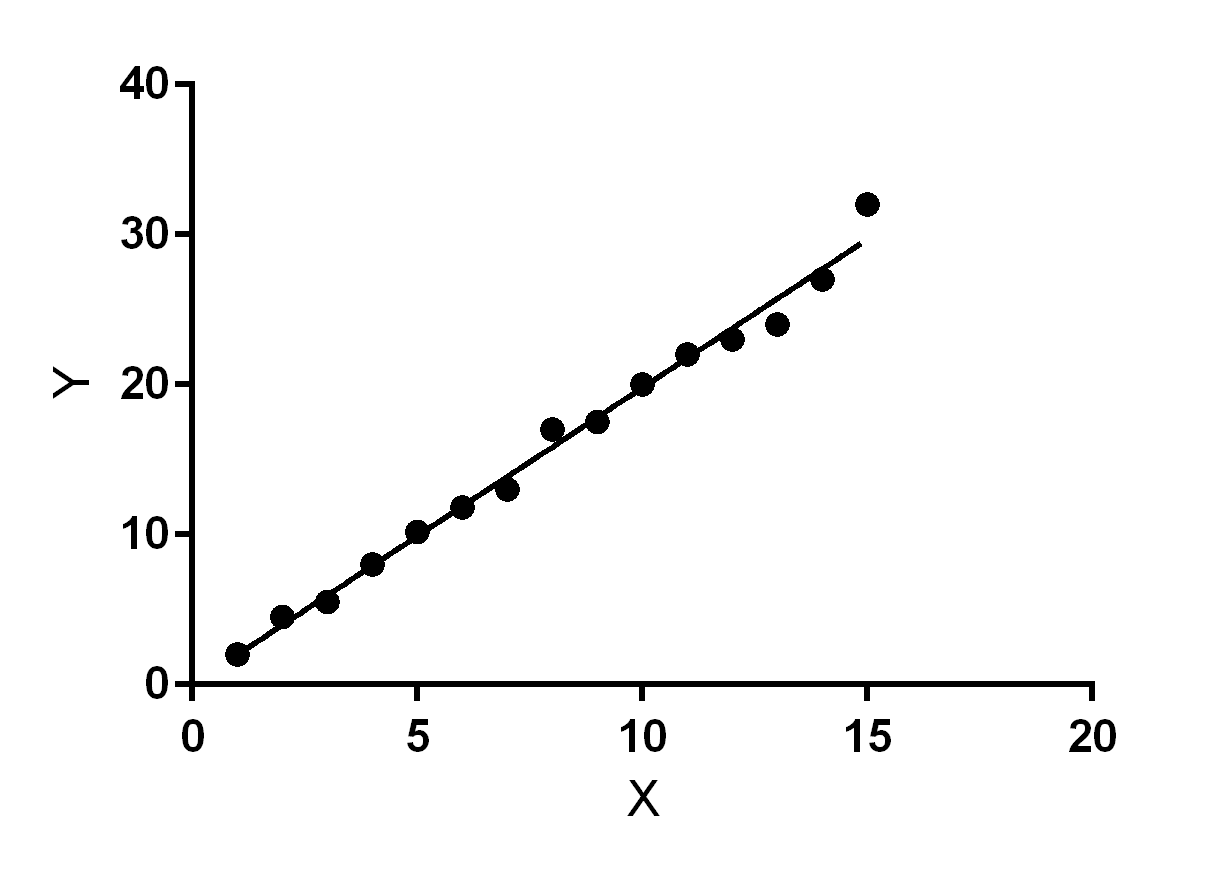
\includegraphics[scale=0.7]{Methods/Linear_regression.png}
      \end{center}
      \caption{Example linear regression}
      \label{fig:linear_regression}
  \end{figure}

  \par The way the independent variables are chosen is usually done by measuring the correlation coefficients between available features in a
  dataset and the target feature and then selecting the features having a high correlation coefficient. Depending on the problem setting, other features can be also considered 
  based on domain knowledge, especially when dealing with a mechanical system as in the case of this work. A good example of this would be the incorporation of 
  the ambient temperature measurement as an input feature---even if it does not highly correlate with the target feature---to make sure that your model generalizes when 
  trying to predict a component's temperature throughout the year, by considering the effect of seasonality 
  (temperatures are expected to be higher in summer than in winter).\\
  In this work, we selected input features based on both domain knowledge and correlation coefficients. We used Kendall's method to measure the rank correlation \cite{Kendall}.
  In contrast to Pearson's correlation coefficient, Kendall's rank correlation can capture both linear and non-linear dependency between two variables by 
  measuring the monotonic relationship. In addition to that, variables don't have to be normally distributed when using Kendall's method.

\subsection{Deep learning}
  Although multiple linear regression models are capable of fitting the data with high accuracy in many applications (e.g., \cite{Linear_Regression_Example_1}), they are,
  by definition, not capable of capturing more complex non-linear dependencies. In addition to that, linear regression may not be appropriate when there are a significant 
  number of independent variables. Deep learning may be a better approach in these situations.\\
  After obtaining better results with it (see Experiment \ref{exp:I}), we decided to train the normal behavior models
  on a feed-forward neural network (for a comprehensive review of deep learning and neural networks, see \cite{Deep_Learning}) having the architecture shown 
  in Fig. \ref{fig:MLP}.

  \begin{figure}[!htbp]
    \begin{center}
      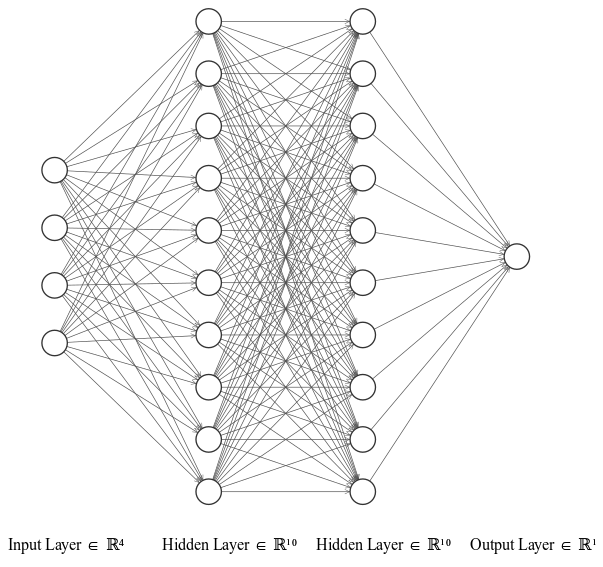
\includegraphics[scale=0.4]{Methods/MLP_cropped.png}
    \end{center}
    \caption{Architecture of normal behavior neural network model used in this work. \\
    \emph{P.S.: The input layer shape will vary based on the experiment and the number of input features.}}
    \label{fig:MLP}
  \end{figure}

  \clearpage
  
\section{Log analysis}
In this section, we will describe the different approaches we propose to utilize SCADA log messages and incorporate them into normal behavior models.
In summary, we introduce three different ways for utilizing SCADA log messages: Extracting input features for normal behavior models, Data filtering, and Visualization of warnings.
We will explain each approach in depth.

\subsection{Extracting input features}
  Most machine-learning architectures can only work with vector-shaped numerical inputs. Given that there are limited resources in the research field on how to generate 
  numerical vectors from wind turbine SCADA system logs (see chapter \ref{chap:soa}), we came up with two methods that were proven capable of not only generating input features for 
  machine-learning normal behavior models but also improving their accuracy (see chapter \ref{chap:experiments}): 1. our Novel method based on domain knowledge and 
  2. Utilizing an open-source framework for analyzing log data called LogPAI. We will discuss each method in detail.

  \subsubsection{Novel method}
    \label{subsub:novel_method}
    \textbf{Background:}\\
    We scanned through the different log messages available in the dataset looking for information that reflects the turbine state and might help the normal behavior model 
    fit the data more accurately. Since normal behavior models monitor the state of a component by monitoring its temperature, we narrowed the search down to operation and system logs
    that reflect events causing a change of temperature in major components. We, then, ended up with a category of logs that shows the states of internal or external ventilators
    of some components (see table \ref{tab:logs}). Being parts of the cooling systems of major components, fans or ventilators must affect the component's temperature.
    \begin{table}[H]
      \centering
      \begin{tabular}{|c|c|}
      \hline
       \textbf{Log text template} & \textbf{Log text sample}\\
       \hline
       Gen. ext. vent. \_, temp:\_\_\_\degree C & Gen. ext. vent. 2, temp:65\degree C \\
       Gen. int. vent. \_, temp:\_\_\_\degree C & Gen. int. vent. 1, temp:50\degree C \\
       HV Trafo. vent. \_, temp:\_\_\_\degree C & HV Trafo. vent. 0, temp:2\degree C \\
       Nac.vent.\_, nac/gear:\_\_\_/\_\_\_\degree C & Nac.vent.3, nac/gear:43/ 54\degree C \\
      \hline
    \end{tabular}
    \caption{Example log text templates with sample texts}
      \label{tab:logs}
    \end{table}

    Indeed, our analysis showed a clear relationship between the state of a ventilator and the temperature of its turbine component.
    As shown in Fig. \ref{fig:vent}, at low temperatures of the generator bearings, the internal ventilator will switch off. The bearings will then heat up which, in turn, causes
    the ventilator to turn on which cools the bearings down, and so on\dots

    \begin{figure}[!htbp]
      \begin{center}
        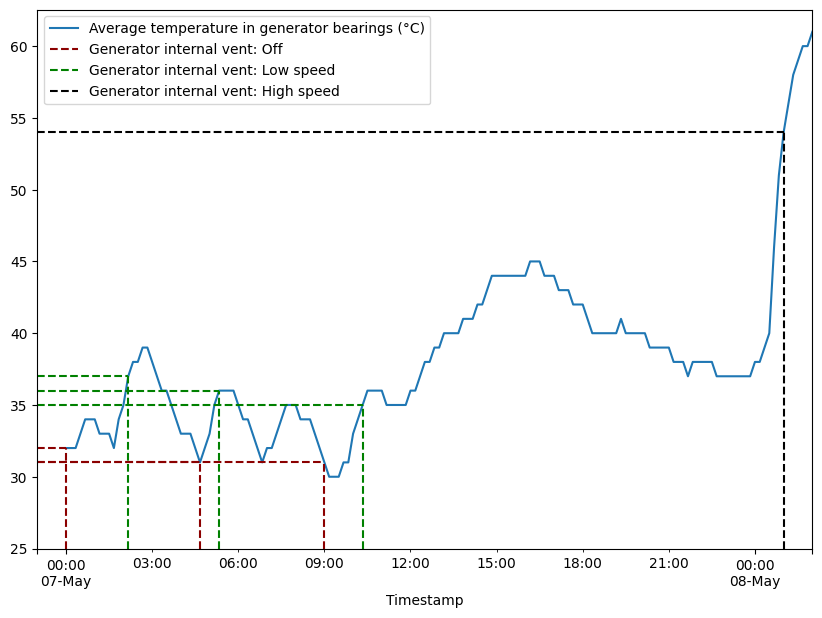
\includegraphics[scale=0.5]{Methods/Vent_Signals.png}
      \end{center}
      \caption{Generator internal vent control signals and their effect on the generator bearings temperature}
      \label{fig:vent}
    \end{figure}

    \begin{flushleft}
      \textbf{Method:}\\
      Analyzing the log texts of interest (e.g., \emph{Gen. ext. vent. 2, temp:65\degree C}), we deduce that they provide three pieces of information: 
      1. Description of the ventilator (e.g., \emph{Gen. ext. vent.}), 2. State of the ventilator (\emph{0, 1, 2 or 3}), 
      3. Temperature of the turbine component the ventilator is installed in (e.g., \emph{65\degree C}).
    \end{flushleft}
    Since the component temperature is regularly provided as a SCADA signal, we decided to focus on the other two parts of the log messages. 
    Our method simply filters log messages containing the word "vent." and creates a new feature for every ventilator (1.) found in the data having its state (2.) as a value.\\
    In contrast to the signals data fixed rate of occurrence (10 min), the generated log feature has an inconsistent frequency (the SCADA system creates a new log entry only 
    when a ventilator changes states). We join both datasets by taking the value of the last occurrence in the log feature vector within a 10-min window relative to a signal reading. 
    Gaps in the log feature columns in the resulting dataset are then filled by propagating the last valid observation forward to the next valid (a ventilator has the same state as long as it hasn't changed).\\
    Measuring the Kendall correlation factor between the generated log features and all the signals of the turbines, we found that for every temperature signal, there is at least 
    one log feature that, on average, highly correlates ($Rank>0.5$) with it.

    \begin{figure}[!htbp]
      \begin{center}
        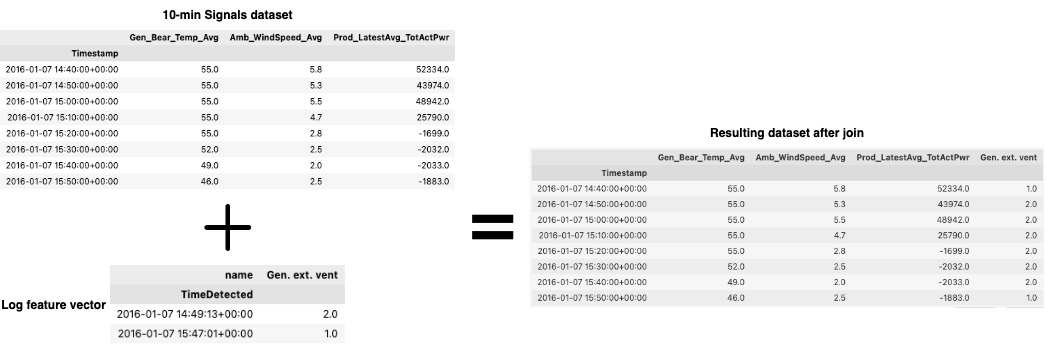
\includegraphics[scale=0.376]{Methods/Log_Merge.png}
      \end{center}
      \caption{Demonstration of the join operation between the signals 10-min dataset and a log feature vector}
      \label{fig:log-merge}
    \end{figure}
    

  \subsubsection{Utilizing LogPAI}
    LogPAI (Log Analysis and Intelligence) is a study project and open-source platform for analyzing and managing log data \cite{LogPAI}. 
    Tsinghua University researchers started the project, which focuses on developing efficient algorithms and tools for log analysis, anomaly detection, and log data visualization.
    LogPAI includes a complete suite of log analysis and processing tools such as Logparser, Loglizer, and Logreduce. 
    These applications can assist users in preprocessing and parsing raw log data, detecting anomalies and patterns, and summarizing log data concisely and understandably.
    We decided to utilize LogPAI's Logparser (\cite{Logparser_1}, \cite{Logparser_2}) and Loglizer (\cite{Loglizer}) to respectively parse and create numerical features from 
    SCADA logs in a more generic and automated way.\\

    \begin{flushleft}
      \textbf{Preprocessing using Logparser:}\\
      From the list of parsers available in the toolkit, we decided to use Drain \cite{Drain} given that it is an online parser, which means it can process the SCADA logs 
      in real-time as they are generated. The Drain algorithm groups similar log messages together and extracts structured events from them using a 
      clustering-based approach. The research demonstrates that Drain is very good at dealing with enormous amounts of log data and extracting meaningful events from 
      noisy and diverse log data. Several phases are involved in the Drain algorithm, including log parsing, log message clustering, and event extraction. 
      Drain employs a fixed-depth tree to parse log messages into a set of log keys and their related values during the log parsing stage. The log keys 
      are unique identifiers for each type of log message, whereas the log values are the specific information connected with each log message. Drain uses a similarity measure 
      to compare the log keys and values of each log message and allocates them to the best appropriate cluster based on their similarity scores during the log message 
      clustering stage. Drain creates a template for each cluster that summarizes the relevant information contained in the log messages once the log messages have been clustered.
      Overall, the Drain algorithm makes an important contribution to log data analysis and management by providing a scalable and effective approach for extracting structured 
      events from unstructured log data.
      Applying Drain on the SCADA log data in hand by specifying its log format "\emph{<TimeDetected>,<TimeReset>,<UnitTitle>,<Content>,<UnitTitleDestination>}", we get 
      output structured log data (see Fig. \ref{fig:logparser} for an example) that the Loglizer can process to generate numerical features.
    \end{flushleft}

    \begin{figure}[!htbp]
      \begin{center}
        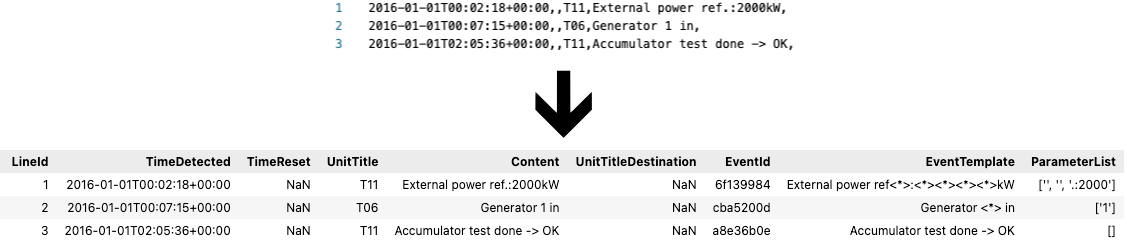
\includegraphics[scale=0.349]{Methods/Logparser.png}
      \end{center}
      \caption{Sample raw logs and their corresponding structured logs after being parsed by Drain}
      \label{fig:logparser}
    \end{figure}

    \begin{flushleft}
      \textbf{Creating numerical features using Loglizer}:\\
      Loglizer's \emph{Feature Extraction} component supports various feature extraction techniques, such as Bag-of-Words, TF-IDF, and Word2Vec, 
      to capture the essential information contained in log data. We utilized the Loglizer feature extractor, using TF-IDF \cite{TF-IDF} for term weighting, to generate numerical 
      features from the parsed logs' \emph{Event IDs}. 
    \end{flushleft}

\subsection{Data labeling and filtering}
  In this approach, we developed a method to improve SCADA-data-driven wind turbine power curve models 
  (for a comprehensive review of the various modeling techniques used to predict the power output of wind turbines and their applications in wind-based energy systems, 
  see \cite{Power_curves}). We start by extracting the log messages that report the current state of operation; namely logs containing one of the following expressions:
  \begin{bulletList}
    \item \emph{"Run"},
    \item \emph{"(Stop|Pause).*kW.*RPM"}, or
    \item \emph{"new SERVICE state"}
  \end{bulletList}
  The SCADA signals are then merged with the extracted log messages, using the same join strategy described in \ref{subsub:novel_method}, and labeled based on the following logic:
  \begin{bulletList}
    \item Turbine's state of operation = \emph{"Run"}, if the log feature contains the expression \emph{"Run"} or \emph{"new SERVICE state: 1"}
    \item Turbine's state of operation = \emph{"Stop"}, if the log feature contains the expression \emph{"(Stop|Pause).*kW.*RPM"} or \emph{"new SERVICE state: 0"}
  \end{bulletList}

  \begin{figure}[!htbp]
    \begin{center}
      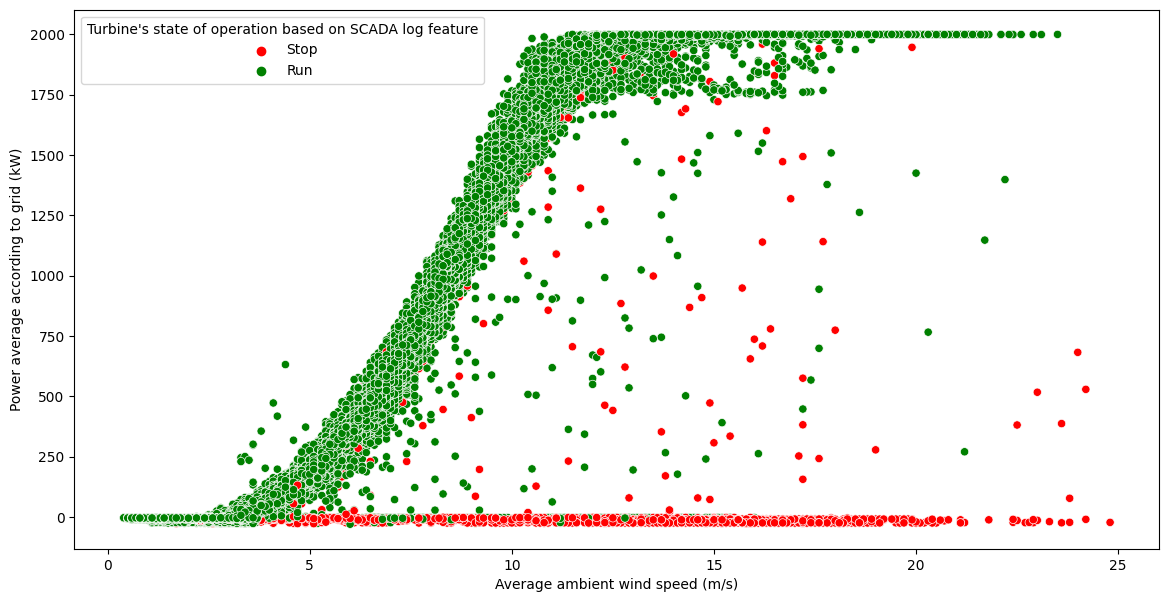
\includegraphics[scale=0.45]{Methods/power_curve.png}
    \end{center}
    \caption{T01 power curve with log-feature-based labels}
    \label{fig:power_curve}
  \end{figure}

  The log-based feature we introduced showed a clear improvement in the accuracy of power curve models (see experiment..TODO) when used to filter the data being input 
  to the normal behavior model (using data points having \emph{"Run"} as the state of operation exclusively).

\subsection{Visualization of warnings}
  Here, we introduced a straightforward yet effective way of visualizing (e.g., on an operation dashboard) messages from the Alarm and Warning logs that are relevant 
  to faults detected or predicted by normal behavior models and that are worth being reported to the operators.\\
  When the normal behavior model detects a fault in a certain turbine component, the SCADA logs are queried for messages reporting high temperatures in this component 
  during the same time window (e.g., last hour, last 12 hours, current day,\dots). If found, these messages could be included in the system reports that get sent to the operators
  to inform them of the detected failure. This gives more visibility and credibility to the detected/predicted failure by the system.\\
  (TODO add graph showing an example)

  \clearpage

\section{Anomaly detection}
  \subsection{Background}
    The main idea behind training and improving normal behavior models is to allow our models to detect anomalies more accurately.
    An anomaly is defined as an occurrence or observation that differs from what is expected, usual, or typical. 
    An anomaly is commonly referred to as an outlier or an uncommon trend in data in numerous domains such as statistics, data analysis, and security.
    By comparing the observed data to a reference set, such as historical data or a pre-defined model, anomalies can be found.
    Positive and negative anomalies are also possible. Depending on the context, positive anomalies could suggest that something is performing better than predicted and 
    negative anomalies indicate that something is underperforming (e.g., in the context of a company's sales figures), or the other way around. In the context of wind
    turbine condition monitoring and when mainly monitoring temperatures of the system, we focus on positive anomalies because a component that is 
    overheating---due to wear and tear, oil leakage, faulty fan,\dots---is likely to fail. There is, however, no unified method in the research field to identify a data point 
    as an anomaly. Brandao et al. (\cite{Brandao_1}, \cite{Brandao_2}) used a fixed value of the mean absolute error as an anomaly threshold in their 
    gearbox and generator fault detection model, even though this number was particular and no longer valid following maintenance procedures. 
    Schlechtingen and Santos \cite{Schlechtingen} used daily average prediction errors in generator bearings temperature to trigger alarms. 
    Zhang and Wang \cite{Zhang_Wang} used a hard threshold of 1.5\degree C for the residual to identify anomalies in the main shaft rear bearing temperature.
    Bangalore and Tjernberg (\cite{Bangalore_1}, \cite{Bangalore_2}, \cite{Bangalore_3}) used a Mahalanobis distance to compare residual and target distributions from 
    the training period to find anomalies in gearbox bearings temperatures. The Mahalanobis distance was averaged over three days and compared to a training result-defined threshold.

  \subsection{Method}
    As there is no standard way to identify anomalies in temperatures in the context of condition monitoring for wind turbines using normal behavior models, we experimented 
    with several methods to do that and, finally, decided to set the anomaly threshold to the maximum prediction error seen in the training period. This way it is 
    guaranteed that the normal behavior models will not label any data point in the training dataset as an anomaly (complying with the assumption that the turbine was operating 
    in a healthy state during the training phase of the model) while having the threshold dynamically set based on the setup (e.g., 
    input and output features, training period, condition of the turbine during the training phase,\dots) without having to incorporate any domain knowledge related to the 
    specific component to-be-monitored. This also helped better compare different architectures of normal behavior models and the effect of incorporating the proposed log features, 
    not only in terms of prediction accuracy but also in terms of the quality and frequency of anomalies identified (a model that better fits the training data will have a 
    tighter anomaly threshold).

  \subsection{Alarms}
    In our approach, we differentiate between \emph{Anomalies} and \emph{Alarms}. An anomaly is a data point that deviates from "normal", whereas an alarm is a proactive 
    way of communication that gets triggered when the operator's attention is urgently needed. The reason why we propose not to send an alarm every time an anomaly is 
    found by the system is that we want our system to limit the number of false alarms as they are costly and counterproductive.\\
    As opposed to anomalies, which are tracked on a 10-min basis, we base alarms on daily events. If the number of anomalies found from the start of a day up until a given 
    point in time exceeds a certain threshold, an alarm is triggered. We set the \emph{alarm threshold} to the 99\textsuperscript{th} percentile of the distribution of the number of 
    anomalies that occurred per day during the training period when using an \emph{anomaly threshold} set as the 99\textsuperscript{th} percentile of the distribution of the 
    training prediction errors. To summarize, an alarm can be defined as an anomaly in the number of system anomalies found per day.\\
    \\
    (TODO: Maybe soma visualization is needed here?)


\section{Summary}
TODO:
PUSH TO THE TOP//
Diagram of all methods put together: ML model + log feature + Anomaly detection + Alarms,...